% ============================================================
% ［架空の記入例・提出不可］研究設定とパラメータはすべて説明用である．
% 通常のchapters/04-method.texには自動で読み込まれない．
% ============================================================
\chapter{提案手法}

\begin{center}
  \UsamiFictionalExampleNotice
\end{center}

\section{全体構成}

本研究では，姿勢推定器自体を再学習せず，推定された関節座標と信頼度から誤推定骨格を除外する．図\ref{fig:method-pipeline}に処理の全体像を示す．入力フレームから既存の姿勢推定器を用いて骨格を求めた後，関節信頼度と骨格辺長の構造的一貫性を統合し，後段処理へ渡す骨格を選択する．この構成により，HRNet\cite{sun2019hrnet}やViTPose\cite{xu2022vitpose}等の推定器を変更せずに適用できる．

\begin{figure}[tb]
  \centering
  % 図ファイルも一式へ収録し，\includegraphicsの使い方を示す．
  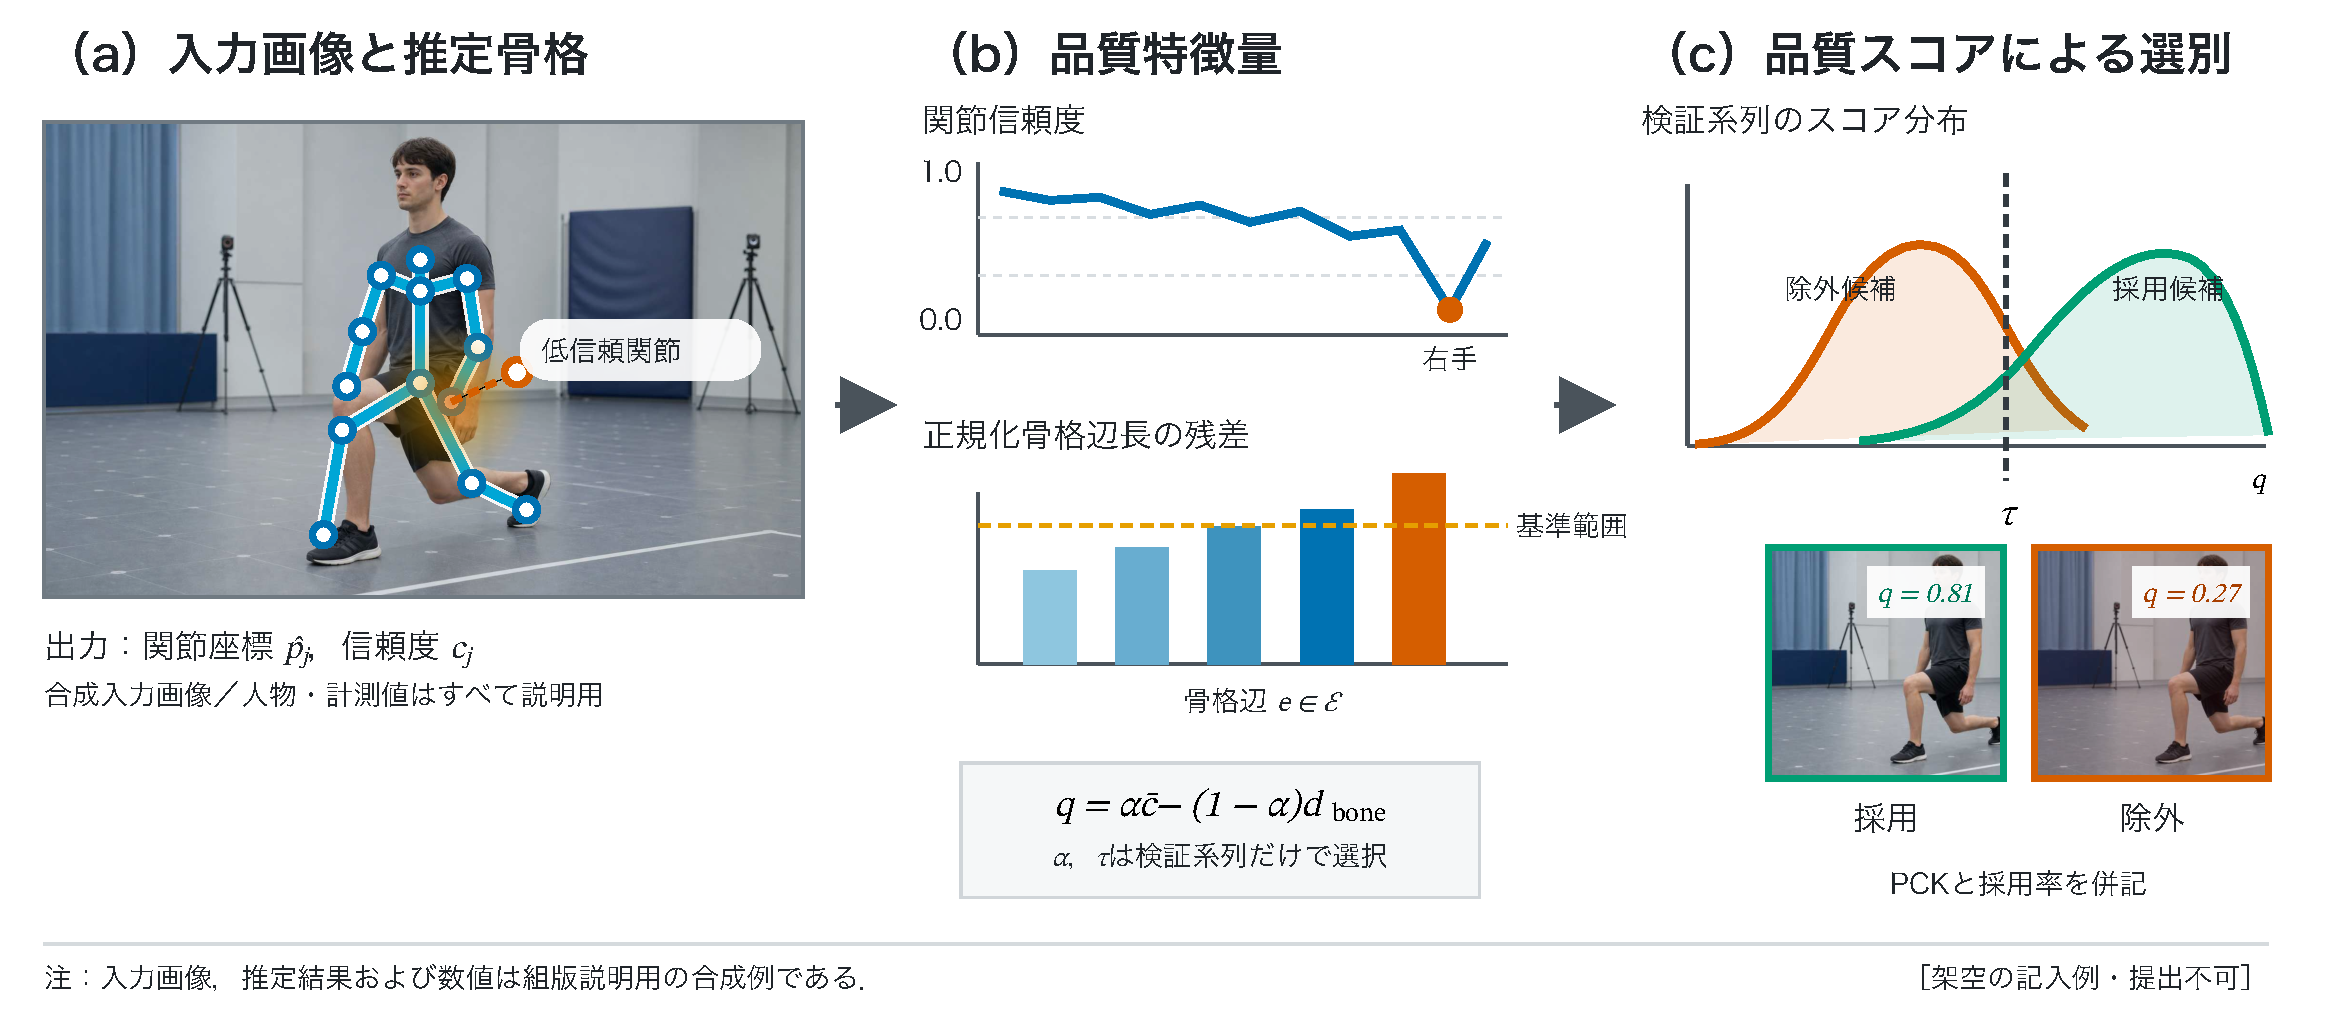
\includegraphics[width=\textwidth]{examples/figures/pose-quality-pipeline.pdf}
  \caption{構造的一貫性を用いた誤推定骨格除外の処理フロー}
  \label{fig:method-pipeline}
\end{figure}

\section{骨格品質スコア}

人物ごとに$J$個の関節を推定し，関節$j$の座標を$\hat{\bm{p}}_j\in\mathbb{R}^2$，信頼度を$c_j\in[0,1]$とする．平均関節信頼度を$\bar{c}=J^{-1}\sum_{j=1}^{J}c_j$とする．また，骨格辺集合を$\mathcal{E}$とし，各辺長を人物の胴体長で正規化した後，学習系列から求めた基準辺長との差の平均を$d_{\mathrm{bone}}$とする．骨格品質スコア$q$を

\begin{equation}
  q=\alpha\bar{c}-(1-\alpha)d_{\mathrm{bone}}
  \label{eq:method-quality-score}
\end{equation}

と定義する．式\eqref{eq:method-quality-score}の第1項は関節単位の確からしさ，第2項は人体構造からの逸脱を表す．$q<\tau$となる骨格を誤推定候補として除外する．この判定は，Part Affinity Fieldsで関節間の対応を扱う方法\cite{cao2017partaffinity}とは異なり，既に構成された骨格の利用可否を判定する後処理である．

\section{実装条件}

記入例では，姿勢推定器をHRNet-W32，入力解像度を$256\times192$画素とした．重み$\alpha$と閾値$\tau$は検証系列のPCK@0.2と採用率の関係から決め，評価系列には触れない．基準辺長は学習系列だけから計算し，左右反転時は関節番号も対応づける．なお，モデル，解像度，データ数およびパラメータは説明用の架空設定である．
